\chapter{Methods}

TODO:\begin{enumerate}
    \item Add in symbol for gaussian process and regressed GP.
\end{enumerate}

\section{Creation of Synthetic Data}

\begin{figure}[htbp]
    \centering
    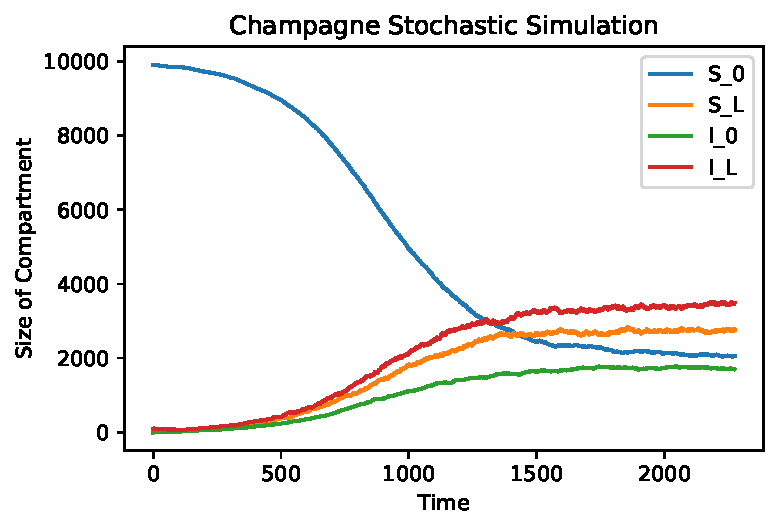
\includegraphics[width=\textwidth]{../champagne_GP_images/champagne_simulation.pdf}
    \caption{
        A Doob-Gillespie Simulation of the model described by
        \cite{champagne_using_2022} with $\alpha = 0.4,$ $\beta = 0.4,$
        $\gamma_L = 1 / 223,$ $\lambda = 0.04,$ $f = 1 / 72,$ $r = 1 / 60,$ and
        $\delta = 0.$ The population was 1000, with 10 initial infections
        (both blood and liver stage).
    }
    \label{fig:champ_doob}
\end{figure}

We investigated the model by \cite{champagne_using_2022} as described in
\ref{sec:champ_mod}. A malaria epidemic was simulated using the Doob-Gillepsie
algorithm (see Figure \ref{fig:champ_doob}), using a population
size of 1,000, and initial infected population of 10 (with both liver and blood
stage infection). The parameters used closely followed those reported in
\cite{champagne_using_2022}: \begin{itemize}
    \item effective blood stage treatment proportion $\alpha = 0.4,$
    \item effective liver stage treatment proportion $\beta = 0.4,$
    \item rate of liver stage disease clearance
          $\gamma_L = 1 / 223 \text{ days}^{-1},$
    \item importation rate $\delta = 0$ (assumed to be known),
    \item rate of infection $\lambda = 0.04 \text{ days}^{-1},$
    \item rate of relapse $f = 1 / 72 \text{ days}^{-1},$
    \item rate of blood stage disease clearance $r = 1 / 60 \text{ days}^{-1}.$
\end{itemize}

From intialisation, the simulation was run for 15,000 events
(with an event being anything that caused the size of any compartment to change
such as an infection, recovery, relapse etc.), after which, the model was
understood to have reached steady state behaviour.

The synthetic data (as summary statistics) measured from the steady state
were:
\begin{enumerate}
    \item $p_\text{obs}:$ the number of currently infected individuals at the
          end of simulated epidemic (steady state prevalence).
    \item $m_\text{obs}:$ the number of cases in the first week of the epidemic
          (first month incidence)
    \item $w_\text{obs}:$ the number of cases in the last week of the epidemic
          (steady state weekly incidence).
\end{enumerate}

New infections which instantly undergo radical cure don't change the size of
each compartment. The number of these `silent' incidences were calculated
between events using a Poisson distribution with rate
$\Delta t \times \alpha \beta \lambda (I_L + I_0) S_0 / N,$ where $\Delta t$ is
the time between events.

\section{Model Simulations and Discrepency Function}

New epidemics were simulated as above, with 15,000 events and at least 30
days (to allow for calculation of incidence in the first month of the
epidemic). For each model run steady state prevalence $p$,
first month incidence $m,$ and steady state weekly incidence $w$ were
calculated with the identical method to the synthetic data.

We defined the discrepency function to be $L_2$ norm of the relative
differences
$$
    \mathcal{D}(\alpha, \beta, \gamma_L, \lambda, f, r)
    := \sqrt{
        \left(\frac{p - p_\text{obs}}{p_\text{obs}}\right)^2
        + \left(\frac{m - m_\text{obs}}{m_\text{obs}}\right)^2
        + \left(\frac{w - w_\text{obs}}{w_\text{obs}}\right)^2
    }.
$$
Relative difference was chosen to limit the impact between the scale
differences of the summary statistics.

\section{Gaussian Process and Initialisation}

We used a Gaussian process as a surrogate model for
$\overline{\ln\mathcal{D}}(\bm{\theta}),$ where
$\overline{\ln\mathcal{D}}(\bm{\theta}),$ was the mean of 30 samples of
$\ln\mathcal{D}(\bm{\theta}).$
We used the kernel
$$
    k(\bm{\theta}_i, \bm{\theta}_i^\prime)
    = \sigma_k^2 (1 + z_i + \frac{z_i^2}{3})\exp(-z_i)
$$
where
$$
    z_i = \sqrt{
        5 \sum_{\theta\in \bm{\theta}}\left(
        \frac{\theta_i - \theta_i^\prime}{\ell_\theta}
        \right)^2
    };
$$ that is, a Mat\'ern kernel with $\nu = 5/2$ and automatic
relevance determination - i.e.\ each parameter $\theta\in\bm{\theta}$ was
scaled by $\ell_\theta.$ This can be seen as giving each parameter its own
length hyperparameter. The Gaussian process was zero mean
with `observation' variance $\sigma^2_o.$

Modelling the mean of the (log) discrepancy function is theoretically more 
sound than modelling the (log) discrepancy function itself, as 
we were not able to find theoretically sound reasons to assume normality,
but the mean is asymptotically normal under reasonable conditions by the
central limit theorem. For example, even under the simplest case that the
discrepency is $L_2$ norm of $k$ differences $x_i$ where
$x_i\sim\mathcal{N}(0, 1),$ $\sqrt{\sum_{i=1}^k x_i^2}\sim\chi(k),$ a Chi 
distribution with $k$ degrees of freedom. 
\textcolor{red}{
    do I need to cite a reference for this distribution (wikipedia)
} 

\begin{table}[htbp]
    \centering
    \begin{tabular}{c |c |c}
        Parameter                                                     & Upper Bound & Unit   \\
        \hline
        Proportion of treatment clearing blood stage disease $\alpha$ & 1           &        \\
        Proportion of treatment clearing liver stage disease $\beta$  & 1           &        \\
        Rate of liver stage disease clearance $\gamma_L$              & 1/30        & 1/days \\
        Rate of infection $\lambda$                                   & 1/10        & 1/days \\
        Rate of relapse $f$                                           & 1/14        & 1/days \\
        Rate of blood stage disease clearance $r$                     & 1/14        & 1/days
    \end{tabular}
    \caption{
        Conservative upper bounds for parameters to be calibrated.
        Values were informed by
        \cite{champagne_using_2022, white_variation_2016}. All lower bounds
        were zero.
    }
    \label{table:param_bounds}
\end{table}

All parameters to be calibrated were given conservative upper bounds after 
considering values reported in the literature, which informed where to define
the Gaussian process. Parameter values outside this range were not considered.

Latin hypercube sampling was used to generate initialise 50 samples of the 
parameter space (scaled to be between zero and the upper bounds described in 
Table \ref{table:param_bounds}). For each set of parameters, 
$\overline{\ln\mathcal{D}}(\bm{\theta})$ was generated. The hyper\-parameters
$\sigma_o^2, \sigma_a^2, \ell_\alpha, \ell_\beta,
    \ell_{\gamma_L}, \ell_\lambda, \ell_f,$
and $\ell_r$ were selected by leave one out cross validation.

\section{Bayesian Acquisition and Parameter Updates}

For 500 iterations, the next $\bm{\theta}$ to sample 
$\overline{\ln\mathcal{D}}(\bm{\theta})$ from
at was found by maximising the expected information acquisition function. 
At each iteration $t,$ 
the gradient descent algorithm was initialised at the sample of $\bm{\theta}$
which minimised the surogate Gaussian process model $\E(d(\bm{\theta})),$ but
with each parameter having a 50\% chance of being initialised uniformly at 
random between it's lower and upper bounds. Each iteration, there was a 
$min\left[1/5 + \exp(1 - t/4), 1 \right]$ probability that one of the
parameters in $\bm{\theta}$ -
$\theta^*$ -
was chosen, and $\overline{\ln\mathcal{D}}(\bm{\theta})$ was sampled at 
$\bm{\theta}$ as well as at 11 evenly spaced values of
$\theta^*.$ $1/5 + \exp(1 - t/4)>1$ for small $t,$ decaying to $1/5$ as $t$ is
large. This was to help initialise the Gaussian process model, as well as
optimise $\ell_\theta.$ Every 50 iterations, the hyperparameters were 
reoptimised using leave one out cross validation. Finally, the synthetic 
likelihood was calculated by $\Pr(d_GP).$

\chapter{Results}

\chapter{Discussion}

multiple runs at once parallelisable

Although most of the procedure we used closely follows the paper by
\cite{gutmann_bayesian_2016}, there are a few key ways in which we modified the
manuscript's method. In particular, we felt the choice of squared exponential
kernel was not a good assumption, since it implicitly assumes a high degree of
smoothness in the target discrepency function. This is unlikely to be met if
the model has any bifurcation points. To compensate for any non-smoothness in
the function, the length scale is forced to be set very small. Therefore,
although the squared exponential is the most commonly chosen kernel,
we used a Mat\'ern kernel with $\nu = 5/2$. This is not as constrained as a
squared exponential kernel, but realisations are twice mean square
differentiable.

A constant mean was used, rather than the quadratic mean, because the
parameters are well bounded, and we don't need to worry about what happens when
they go to infinity. Post-hoc mean fitting could be done on the discrepencies
sampled space in order to extend the likelihood into regions that haven't been
tested without reverting to the mean function.

There seems to be a mistake in \cite{gutmann_bayesian_2016}, where the
exploration parameters is written as
$\eta_t:= \sqrt{2\ln(\frac{t^{2d + 2}\pi^2}{3\varepsilon})}.$ This seems to be
inherited from \cite{brochu_tutorial_2010}. We use Brochu's original citation
\cite{srinivas_gaussian_2010} to revise this to
$\eta_t:= \sqrt{2\ln(\frac{t^{2d + 2}\pi^2}{3\varepsilon})}.$
\footnote{One Python package that implements BOLFI notes this error, see:
    \url{https://github.com/elfi-dev/elfi/blob/dev/elfi/methods/bo/acquisition.py}}

The Gaussian process and Gaussian process regression was implemented using
TensorFlow in Python \cite{abadi_tensorflow_2015}.

\section{Results}

